\documentclass[a4paper,12pt]{article}
\usepackage{times}
\usepackage{hyperref}
\usepackage{xcolor}
\usepackage{graphicx}

\usepackage{geometry}
\geometry{
    a4paper,
    margin=1in,
 }

\usepackage{listings}
\usepackage{xcolor}

\definecolor{codegreen}{rgb}{0,0.6,0}
\definecolor{codegray}{rgb}{0.5,0.5,0.5}
\definecolor{codepurple}{rgb}{0.58,0,0.82}
\definecolor{backcolour}{rgb}{0.95,0.95,0.92}

\lstdefinestyle{mystyle}{
    language=scala,
    backgroundcolor=\color{backcolour},   
    commentstyle=\color{codegreen},
    keywordstyle=\color{magenta},
    numberstyle=\tiny\color{codegray},
    stringstyle=\color{codepurple},
    basicstyle=\ttfamily\footnotesize,
    breakatwhitespace=false,         
    breaklines=true,                 
    captionpos=b,                    
    keepspaces=true,                 
    numbers=left,                    
    numbersep=5pt,                  
    showspaces=false,                
    showstringspaces=false,
    showtabs=false,                  
    tabsize=2
}

\lstset{style=mystyle}

\hypersetup{
    colorlinks,
    citecolor=black,
    linkcolor=black,
    urlcolor=black
}

\begin{document}

\begin{titlepage}
    \begin{center}
        \vspace*{1cm}
 
        \LARGE
        \textbf{Lab 2: FIR Filter with Generators}
 
        \vspace{0.5cm}

        \large
        CS4362 - Hardware Description Languages
             
        \vspace{1.5cm}
 
        \textbf{190332D\\Sasitha Kumarasinghe}
 
        \vfill
            
        \normalsize
        Department of Computer Science and Engineering\\
        University of Moratuwa\\
        \today
             
    \end{center}
 \end{titlepage}

\section{Implementation}

The implementation was done using \lstinline|chisel3| 3.5.6 library with Scala 2.12.17. The parameters \lstinline|taps: Seq[SInt]| and \lstinline|bitWidth: Int| were used to parameterize the FIR filter. An intermediate register array \lstinline|buffer: Vec[SInt]| was used to store the input sequence. The output was calculated by multiplying the taps with the buffer values and summing them up using the \lstinline|reduce| method of \lstinline|muls: Vec[SInt]|. Finally, the output was assigned to \lstinline|io.out|. The \lstinline|Utils.readCoefficients| function was implemented to read the coefficients from a CSV file. The \lstinline|Utils.emitVerilog| function was implemented to generate the Verilog code for the FIR filter.

\vspace{0.3cm}

\noindent
The listing \ref{lst:fir} shows the implementation of the FIR filter.

\vspace{0.3cm}

\begin{lstlisting}[caption={FIR Filter},captionpos=b,label={lst:fir}]
class FirFilter(bitWidth: Int, taps: Seq[SInt]) extends Module {
  val io = IO(new Bundle {
    val in = Input(SInt(bitWidth.W))
    val out = Output(SInt())
  })

  val buffer = Reg(Vec(taps.length, SInt(bitWidth.W)))
  buffer(0) := io.in
  for (i <- 1 until taps.length) {
    buffer(i) := buffer(i-1)
  }

  val muls = VecInit.tabulate(taps.length)(i => taps(i) * buffer(i))

  io.out := muls.reduce(_ +& _)
}
\end{lstlisting}

\vspace{0.3cm}

\noindent
Figures \ref{fig:lowpass}, \ref{fig:highpass} and \ref{fig:bandpass} show the block diagrams of sample FIR filter instances for low pass, high pass and band pass respectively.

\begin{figure}[ht]
    \centering
    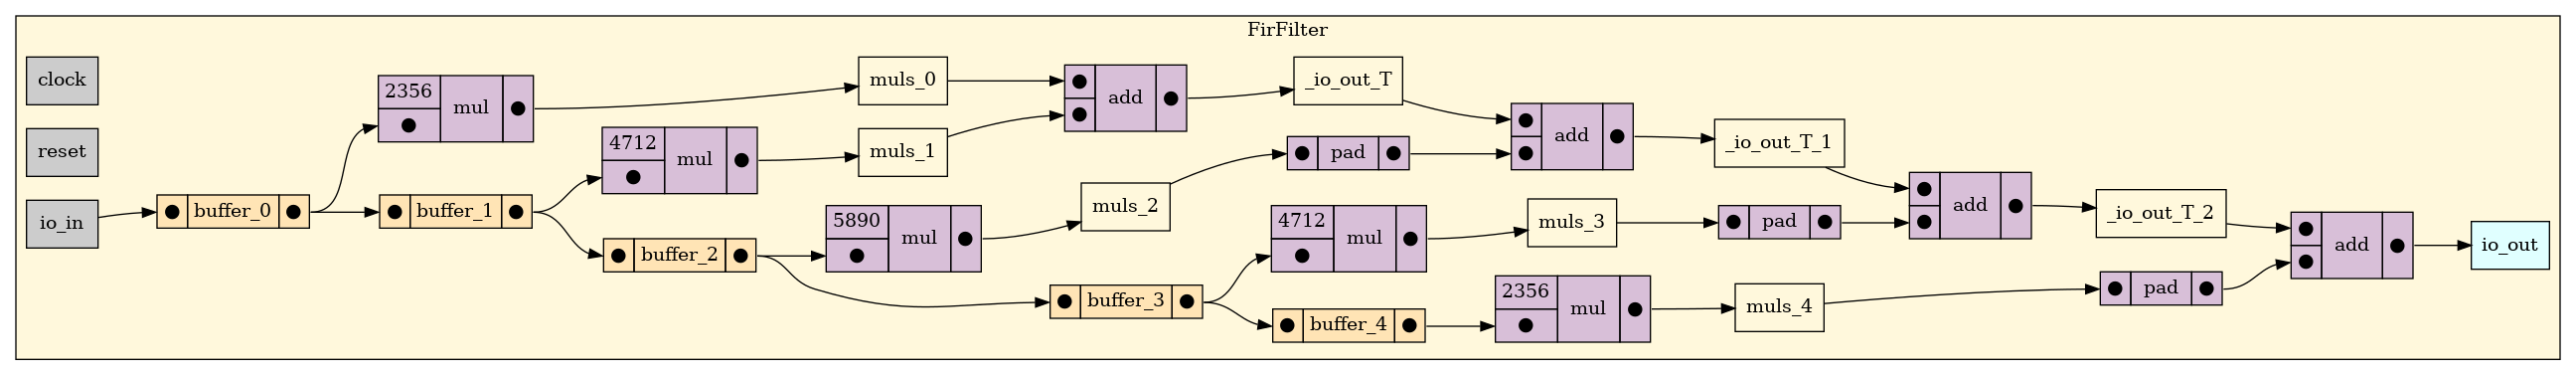
\includegraphics[width=\textwidth]{images/lowpass.png}
    \caption{Low Pass FIR Filter}
    \label{fig:lowpass}
\end{figure}

\begin{figure}[ht]
    \centering
    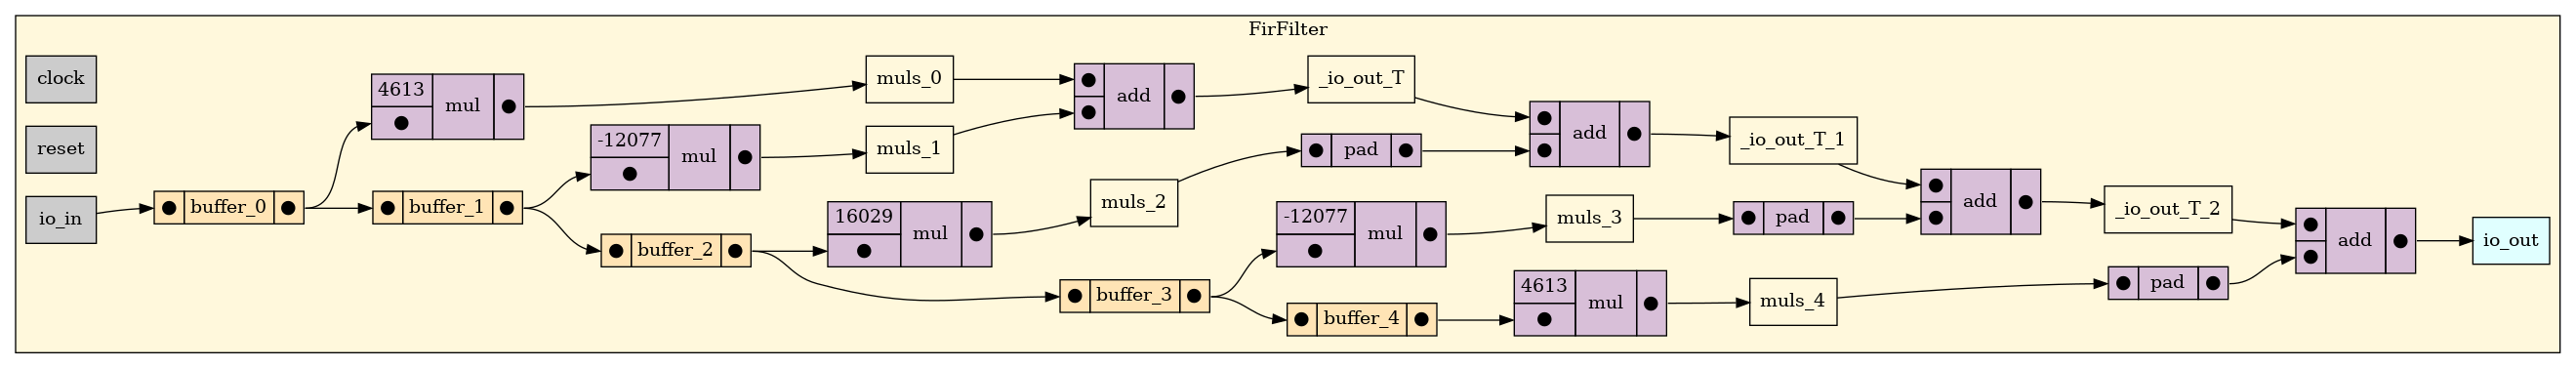
\includegraphics[width=\textwidth]{images/highpass.png}
    \caption{High Pass FIR Filter}
    \label{fig:highpass}
\end{figure}

\begin{figure}[ht]
    \centering
    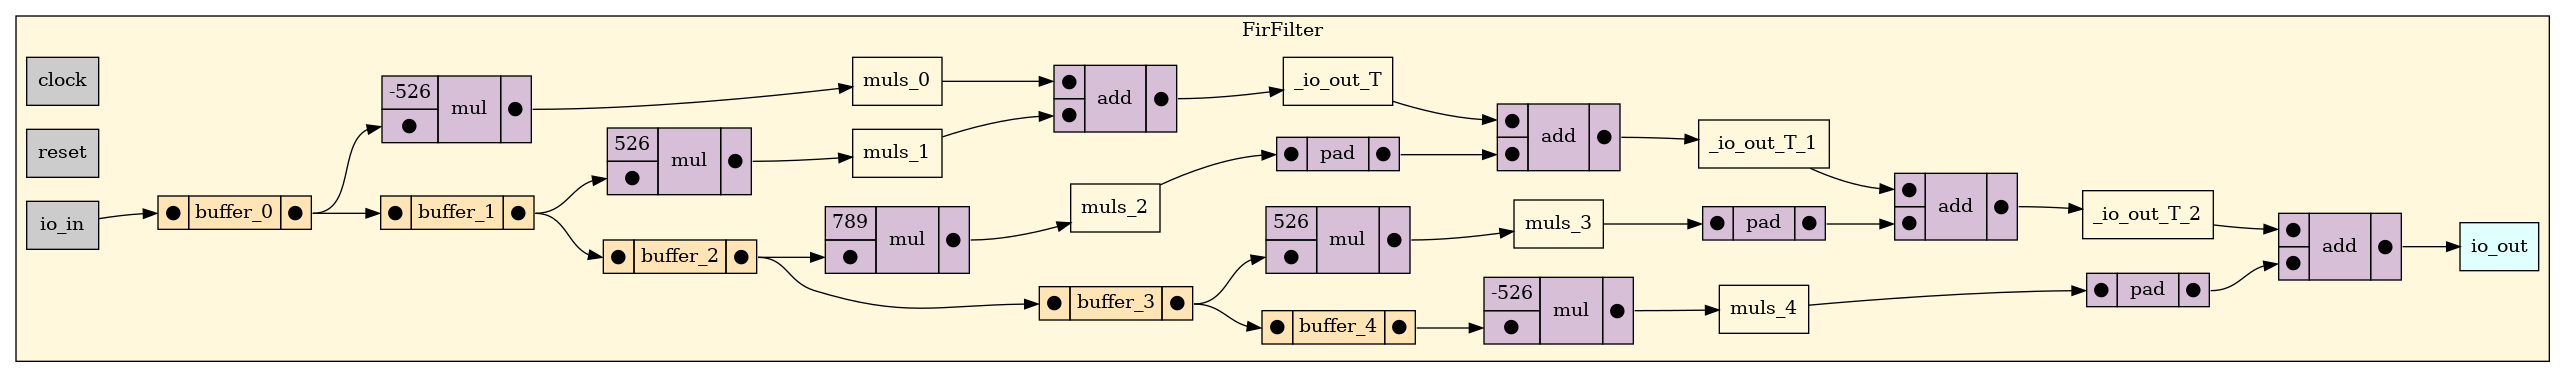
\includegraphics[width=\textwidth]{images/bandpass.png}
    \caption{Band Pass FIR Filter}
    \label{fig:bandpass}
\end{figure}

\section{Testing}

Testing was done with \lstinline|chiseltest| library. The FIR Filter was configured with 25 16-bit-wide taps. The input sequence was defined as a 3-cycle sine wave. The output was compared with the expected output. The listing \ref{lst:testbench} shows the implementation of the testbench. The test result is shown in figure \ref{fig:testbench}.

\vspace{0.3cm}

\begin{lstlisting}[caption={Testbench},captionpos=b,label={lst:testbench}]
class FirFilterTest extends AnyFlatSpec with ChiselScalatestTester {
  "FirFilter" should "PASS" in {
    val bitWidth = 16
    val coeffs = Seq(
      621.S(bitWidth.W), 1252.S(bitWidth.W), 955.S(bitWidth.W),
      -464.S(bitWidth.W), -1427.S(bitWidth.W),
      -442.S(bitWidth.W), 1279.S(bitWidth.W), 815.S(bitWidth.W),
      -2028.S(bitWidth.W), -2978.S(bitWidth.W),
      1849.S(bitWidth.W), 9985.S(bitWidth.W), 14052.S(bitWidth.W),
      9985.S(bitWidth.W), 1849.S(bitWidth.W),
      -2978.S(bitWidth.W), -2028.S(bitWidth.W), 815.S(bitWidth.W),
      1279.S(bitWidth.W), -442.S(bitWidth.W),
      -1427.S(bitWidth.W), -464.S(bitWidth.W), 955.S(bitWidth.W),
      1252.S(bitWidth.W),621.S(bitWidth.W)
    )
    test(new FirFilter(bitWidth, coeffs)) { c =>
      // To simulate a sine wave of 3 cycles
      val inputs = Seq(
        0.S, 23166.S, 32767.S, 23166.S, 0.S, -23166.S, -32768.S, -23166.S,
        0.S, 23166.S, 32767.S, 23166.S, 0.S, -23166.S, -32768.S, -23166.S,
        0.S, 23166.S, 32767.S, 23166.S, 0.S, -23166.S, -32768.S, -23166.S
      )
      // Expected outputs of the FIR filter
      val expectedOutputs = Seq(
        0.S, 14386086.S, 49352139.S, 77533900.S, 49547293.S,
        -40524326.S, -117099665.S, -95446734.S,
        1001663.S, 49878561.S, 540937.S, -6280916.S, 221906448.S,
        645662149.S, 922528801.S, 701824145.S,
        999814.S, -747399325.S, -1039099553.S, -692478191.S,
        49544165.S, 729480385.S, 971343458.S, 666331319.S
      )
      for ((input, expectedOutput) <- inputs.zip(expectedOutputs)) {
        c.io.in.poke(input)
        c.clock.step(1)
        c.io.out.expect(expectedOutput)
      }
    }
  }
}
\end{lstlisting}


\begin{figure}[ht]
    \centering
    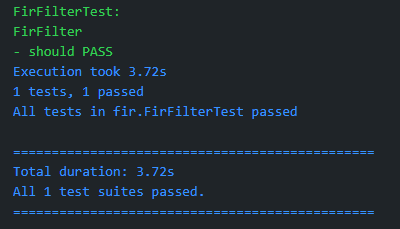
\includegraphics[width=0.7\textwidth]{images/testbench.png}
    \caption{Test results}
    \label{fig:testbench}
\end{figure}

\end{document}
